\documentclass[xcolor=table]{beamer}
\usetheme{Madrid}
\usecolortheme{beaver}

%%%%%%%%%%%%%%%%%%%%%%%%%%%%%%%%%%%%% FOR FSM %%%%%%%%%%%%%%%%%%%%%%%%%%%%%%%%%%%%%%%%%%%%%%%%
\usepackage{tikz}
\usetikzlibrary{automata, positioning, arrows}
\tikzset{
  ->, % makes the edges directed
  >=stealth', % makes the arrow heads bold
  node distance=3cm, % specifies the minimum distance between two nodes. Change if necessary.
  every state/.style={thick, fill=gray!10}, % sets the properties for each ’state’ node
  initial text=$ $, % sets the text that appears on the start arrow
}
%%%%%%%%%%%%%%%%%%%%%%%%%%%%%%%%%%%%% FOR FSM %%%%%%%%%%%%%%%%%%%%%%%%%%%%%%%%%%%%%%%%%%%%%%%%

\title[Sequence Detector]
{Sequence Detector}
\subtitle{DCS Final Presentation}
\institute{DTU}
\author{Jatin Pandey \& kumood}
\logo{
  \includegraphics[height=1cm]{./src/logo.png}
}
\begin{document}
  \frame {
      \titlepage
    }
  \frame {
      \frametitle{What is a Sequence Detector?}
      A sequence detector accepts as input a string of bits: either 0 or 1.   Its output goes to 1 when a target sequence has been detected.
    }
  \frame{
      \frametitle{Types of Sequence Detector}
      There are two basic types of Sequence Detector
      \begin{itemize}
        \item Overlap
        \item Non-Overlap
      \end{itemize}
    }
  \frame{
      \frametitle{Simple Finite State Machine}
      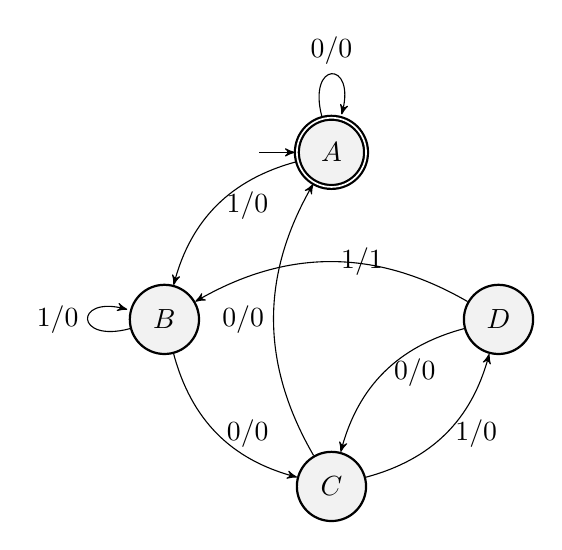
\begin{tikzpicture}
        \node[state, initial, accepting] (1) {$A$};
        \node[state, below left of=1] (2) {$B$};
        \node[state, below right of=2] (3) {$C$};
        \node[state, above right of=3] (4) {$D$};

        \draw (1) edge[above, bend right, right = 0.1] node{$1/0$} (2)
        (1) edge[loop above] node{$0/0$} (1)
        (2) edge[loop left] node{$1/0$} (2)
        (2) edge[below, bend right, right = 0.1] node{$0/0$} (3)
        (3) edge[left, bend left,left=0.2] node{$0/0$} (1)
        (3) edge[below, bend right, right = 0.2] node{$1/0$} (4)
        (4) edge[below, bend right, right = 0.2] node{$0/0$} (3)
        (4) edge[right, bend right, right = 0.2] node{$1/1$} (2);
    \end{tikzpicture}
    }
  \frame{
      \frametitle{State Table}
      Generating State Table with outputs
      \begin{table}[]
\begin{tabular}{|c|c|l|c|l|}
\hline
\rowcolor[HTML]{FFCCC9} 
Present State & \multicolumn{4}{c|}{\cellcolor[HTML]{FFCCC9}Next State / Output}                                        \\ \hline
\rowcolor[HTML]{FFCCC9} 
              & \multicolumn{2}{c|}{\cellcolor[HTML]{FFCCC9}X = 0} & \multicolumn{2}{c|}{\cellcolor[HTML]{FFCCC9}X = 1} \\ \hline
\rowcolor[HTML]{FFFFFF} 
A             & \multicolumn{2}{c|}{\cellcolor[HTML]{FFFFFF}A/0}   & \multicolumn{2}{c|}{\cellcolor[HTML]{FFFFFF}B/0}   \\ \hline
\rowcolor[HTML]{FFFFFF} 
B             & \multicolumn{2}{c|}{\cellcolor[HTML]{FFFFFF}A/0}   & \multicolumn{2}{c|}{\cellcolor[HTML]{FFFFFF}C/0}   \\ \hline
\rowcolor[HTML]{FFFFFF} 
C             & \multicolumn{2}{c|}{\cellcolor[HTML]{FFFFFF}D/0}   & \multicolumn{2}{c|}{\cellcolor[HTML]{FFFFFF}C/0}   \\ \hline
\rowcolor[HTML]{FFFFFF} 
D             & \multicolumn{2}{c|}{\cellcolor[HTML]{FFFFFF}A/0}   & \multicolumn{2}{c|}{\cellcolor[HTML]{FFFFFF}E/0}   \\ \hline
\rowcolor[HTML]{FFFFFF} 
E             & \multicolumn{2}{c|}{\cellcolor[HTML]{FFFFFF}A/0}   & \multicolumn{2}{c|}{\cellcolor[HTML]{FFFFFF}C/1}   \\ \hline
\end{tabular}
\end{table}
  }
\end{document}
